\documentclass[11pt,a4paper]{article}
\usepackage[T1]{fontenc}
\usepackage[utf8]{inputenc}
\usepackage{lmodern}
\usepackage{amsmath,amssymb,amsthm,mathtools,mathrsfs}
\usepackage{graphicx,float,xcolor,multicol}
\usepackage[shortlabels]{enumitem}
\usepackage[margin=27mm]{geometry}
\usepackage{microtype,needspace,placeins}
\usepackage{tikz,tikz-cd}
\usetikzlibrary{arrows.meta,calc,positioning,patterns,decorations.pathreplacing}
\usepackage[colorlinks=true,linkcolor=teal,urlcolor=teal,citecolor=teal]{hyperref}
\setlength{\parindent}{0pt}
\setlength{\parskip}{.6em}
\setcounter{secnumdepth}{0}
\allowdisplaybreaks
\raggedbottom
\providecommand{\cross}{\times}
\DeclareUnicodeCharacter{2020}{\ensuremath{\dagger}}
\DeclareMathOperator{\supp}{supp}
\DeclareMathOperator*{\esssup}{ess\,sup}
\providecommand{\chapter}{\section}
\newenvironment{tool}[2]{\subsection*{Tool #1 --- #2}}{}
\newcommand{\ToolRef}[1]{Tool #1}
\newcommand{\FigureTag}[2]{\textit{Figure #1}}
\newcommand{\Result}[1]{\subsection*{#1}}
\newcommand{\Application}[1]{\subsubsection*{Application\if\relax\detokenize{#1}\relax\else\space--- #1\fi}}
\newcommand{\ProofHeading}{\par\textit{Proof.}\space}
\newcommand{\ProofOf}[1]{\par\textit{Proof of #1.}\space}
\newcommand{\RemarkHeading}{\par\textbf{Remark.}\space}
\newcommand{\NoteHeading}{\par\textbf{Note.}\space}
\newcommand{\ExerciseHeading}{\par\textbf{Exercise.}\space}

\graphicspath{{figures/k-theory/}}
\begin{document}
\section*{Locally Trivial Bundles}
% BLOG-CONTENT-BEGIN
\section{Introduction}


Our goal in this series is to understand homotopy theory on the category of topological spaces. To give an analogy of how one attempts to achieve this, consider $\text{Sets}$. To classify objects in $\text{Sets}$ one defines an "algebraic" invariant $\text{card}(X)$ for $X \in \text{Ob}(\text{Sets})$ satisfying:-

\begin{enumerate}
    \item $\text{card}\big(X \bigsqcup Y\big)) = \text{card}(X) + \text{card}(Y)$
    \item $\text{card}(X) = \sup_{F \subseteq_{\text{finite}} X}{\big\{\text{card}(F)\big\}}$
\end{enumerate}
Then, as finite objects in $\text{Sets}$ are generated by finite colimits of $\{*\}$, and countable objects by colimits of finite sets; the function
$\text{card}$ is completely determined by its value on the final object $\{*\}$. Said differently, the counting axioms (1) and (2) of the "algebraic" invariant impersonate the way sets are constructed out of simpler sets. With $\text{card}(\{*\}) = 1$, one can classify countable objects in $\text{Sets}$ upto bijections by "counting" the number of elements in it (dictated explicitly by (1) and (2)). We intend to mimick the same in the category $\text{Top}$. To do so, we search for homotopy invariants, (i.e.) algebraic objects that count certain features indicative of the topological structure that remain invariant under continuous deformations. This leads us to two very basic questions: count what? and count how?

Following Poincar\'e one can begin by looking at loops upto homotopy equivalences, captured by the groups $\{\pi_n(X, x_0)\}_n$. These groups in general don't satisfy nice counting axioms, in particular, they don't satisfy what's called an Excision Axiom: One must facilitate these groups with spaces (preferably CW-complexes) that are $\infty$-connected for them to add up like so: $\pi_n\big(X\bigvee Y, (x_0, y_0)\big) \cong \pi_n(X)\oplus \pi_n(Y)$. To overcome this problem one must come up with new ways to count, put differently one must build objects in topological spaces in ways not involving sticking two spaces together, which won't take us far. Further, homotopy groups do have redeeming qualities captured by the following:-
\subsection*{Theorem — Whitehead}Let $f:X \rightarrow Y$ be a map between CW-complexes, if $f$ induces an isomorphism between all homotopy groups of $X$ and $Y$, then $X\sim Y$.  

\subsection*{Theorem — Cellular Approximation}Every topological space $X$ is weakly homotopy equivalent to a CW-complex.


The above two theorems tell us that homotopy groups almost classify all topological spaces upto continuous deformations; hence one can't entirely abandon them in search for better invariants. So, one looks for algebraic invariants satisfying solid counting axioms with some revealing connections to the homotopy group. This brings us to a very promising candidate: Eilenberg-Steenrod Axioms (ESA). (Co)homology theories are essentially theories around a family of algebraic invariants satisfying ESA. It is illuminating to be acquainted with ESA by tracing how the axioms impersonate the way spaces are built out of simpler spaces. Suppose you have a sequence of functors $\{H_n\}_n$ from the category of pair of topological spaces Top(2) to $\mathbb{Z}$-modules, the following list captures how some the various generalized counting procedures hit on the foundational building machinery in Top.


\begin{enumerate}[(I)]
    \item $f\sim g$ implies $H_n(f) = H_n(g)$ $\longleftrightarrow$ $X\sim Y$ implies $X = Y$.
    \item $H_n(X\setminus U, A\setminus U)\cong H_n(X, A)$ $\longleftrightarrow$ removing $U\subseteq \text{Int}(A)$ from $X$.
    \item $H_n(*) = 0$ $\longleftrightarrow$ $\{*\}$ is the null space.
    \item $H_n\bigg(\coprod\limits_{\alpha}X_{\alpha}\bigg)\cong \bigoplus\limits_{\alpha}H_n(X_{\alpha})$ $\longleftrightarrow$ disjoint union of spaces.
    \item $H_n(X\times Y) \cong \bigoplus\limits_{i+j=k}H_i(X)\otimes H_j(Y)$ $\longleftrightarrow$ products of spaces.
\end{enumerate}


Present literature is loaded with such functors counting features like number of $n$-holes in a space $X$ (singular homology), or number of closed forms upto exactness on a smooth manifold (de Rham cohomology), along with its generalized counterparts in sheaf (co)homology. Even the homotopy groups satisfy many in the list above. Regardless, these counting axioms don't capture the general ways of constructing spaces in Top, hence are far from classifying them. 


Around 1950s, inspired by Grothendieck's work on Riemann-Roch Theorems on algebraic varieties, Atiyah introduced for a space $X$, the "ring of complex vector bundles" $K(X)$ to obtain differentiable analogues of Riemann-Roch Theorems \cite{atiyah1959riemann}. Using Bott periodicity for the infinite unitary group he constructed a "periodic" cohomology theory, now called \textbf{K-theory}; (i.e.) he constructed a sequence of functors with requisite natural transformations satisfying all but one Eilenberg-Steenrod Axiom. He then answered questions for the K-theory on homogeneous spaces which for ordinary cohomology theories have successful treatment. Further, it has been illustrated by mathematicians like Hirzebruch, Atiyah, Singer and Adams that this new cohomology theory can be applied to various topological questions giving better results than any known ordinary cohomology theory. We state some of those results here:- 
\subsection*{Theorem — Frobenius Conjecture}The following is true only for $n \in \{1,2,4,8\}$:-
\begin{enumerate}[(i)]
    \item $\mathbb{R}^n$ is a division algebra \cite{milnor1958some}.
    \item $S^{n-1}$ is parallelizable \cite{atiyah1961bott}. 
\end{enumerate}

\subsection*{Theorem — Atiyah-Singer Index Theorem}For an elliptic differential operator $D$, the analytic and topological indices are same \cite{atiyah1968bott}.

This brings us to the raison d’\^etre of this series. We shall begin by introducing the basic objects of study - fibre bundles; then we shall specialize to what are called \href{https://codezen1729.github.io/math-blog/\#/post/vector-bundles}{complex vector bundles}, and illustrate \href{https://codezen1729.github.io/math-blog/\#/post/bott-periodicity-k-theory}{Atiyah's construction of K-theory} on compact Hasudorff spaces. There on, the reader shall be sufficiently equipped to take up any of the directions pointing towards the preceding two theorems.

% RESTORED-INTRO-END

\section{Locally Trivial Bundles}


The language of vector bundles, or in general locally trivial fibre bundles helps in inducing global structures on a space $B$, if one \textit{appropriately} replaces points in it (locally) by objects from certain categories; illustrated by the following few classical instances:-


\begin{enumerate}[(i)]
    \item Let $B$ be a smooth manifold; replacing points $b \in B \text{ by the space } T_bB^* \otimes T_bB^*$
    yields the idea of integrability, lengths, angles, curvature, all subsumed in its generality by the structure of a Riemannian manifold on $B$.
    
    \item If $B$ were a topological manifold then replacing points $b \in B \text{ by } \mathbb{R}^{\text{dim}(B)}$ gives orientability, rank theorems, paving way for differential geometry on $B$.
    
    \item If $B$ were a $G$-space then putting $G  \text{(a topological group) in place of points }b\in B$ would give us regular covering spaces over $B$, or in general, the theory of principal $G$-bundles.
    
    \item We shall focus on $B$ (a topological space) with points $b \in B \text{ replaced by } F$ (another topological space) leading one to the theory of fibrations (or fibre bundles) \cite{fomenko2016homotopical}.
\end{enumerate}

Although the pragmatic reason given above to study fibre bundles should do the job of justifying its presence in the mathematics we share - an attempt to give a more systematic "hands-on" reason to do the same is worthwhile: Given a space $E$, we aspire to understand topology and analysis on it via simpler spaces. We have at our disposal two basic categorical constructions: limits and colimits. These constructions in itself can be quite fuzzy; adhering to our goal of simplification we shall focus on its elementary instances: products (or fibred products) and disjoint unions (or fibred coproducts). We shall construct (and study) spaces $E$ via products and disjoint unions of simpler spaces $\{U_{\alpha}\}_{\alpha}$ and $F$; which in a nutshell happens to be the foundational philosophy of bundle theory. Having motivated the object of study, let us introduce it formally. Further details can be found in \cite{luke2013vector}.

\subsection*{Definition 2.1 — Locally Trivial Bundle} Given a map $p: E \xrightarrow{} B$ between spaces $E$ and $B$. A \textbf{locally trivial bundle} $\eta = (E, B, F, p)$ is the following data:-

\begin{enumerate}[(i)]
    \item $F$, a topological space.
    
    \item $p^{-1}(b) \cong F   (\forall b, b \in B)$
    
    \item $\forall b \in B, \exists  U_b$, a neighbourhood of $b$, and a homeomorphism $\varphi_b$ such that the following commutes:- 
 
  $$\begin{tikzcd}[column sep = large, row sep = large]
        p^{-1}(U_b) \arrow[rd, "p"'] 
        && U_b \cross F \arrow[ld, "\pi"] \arrow[ll, "\varphi_b"'] \\
        & U_b
    \end{tikzcd}$$


where $\pi(u, f):= u$, is the canonical projection.
\end{enumerate} 

Furthermore, 

\begin{itemize}
    \item F is called the \textbf{fibre} of $p$.
    \item $\{\varphi_{\alpha}\}_{\alpha}$ are called the \textbf{(local) trivializing maps} for $E$.
    \item $\{U_{\alpha}\}_{\alpha}$ is called the \textbf{(locally) trivializing open cover} of $B$.
    \item $B$ and $E$ are called the \textbf{base space} and the \textbf{total space} (respectively).
    \item $p$ is called the \textbf{bundle map}.
    \item $\varphi_{\alpha \beta}:= \varphi_{\alpha}^{-1}\circ \varphi_{\beta}$, a self map on $(U_{\alpha}\cap U_{\beta})\times F$, are called \textbf{transition functions}.
\end{itemize}

In simple words, fibre bundles $(E, B, F, p)$ are continuously varying family of spaces modeled by $E$, mutually homeomorphic to $F$, over $B$. With the special case $F = \{*\}$, one recovers the usual notion of continuity between spaces.

Given $B$, $F$, a trivializing cover $\{U_{\alpha}\}_{\alpha}$ of $B$, and transition functions $\{\varphi_{\alpha \beta}\}_{\alpha, \beta}$ satisfying:- 
\begin{enumerate}[(i)]
    \item $\varphi_{\alpha \alpha} \equiv \text{Id}$.
    \item $\varphi_{\alpha \beta}\circ \varphi_{\beta \gamma}\circ \varphi_{\gamma \alpha} \equiv \text{Id}$ (in particular, $\varphi_{\alpha \beta}\circ \varphi_{\beta \alpha} \equiv \text{Id}$).
    \item $\varphi_{\alpha \beta}(x, f) = (x, f')$ ((i.e.) $\varphi_{\alpha \beta}$ is a fibre preserving map).
\end{enumerate}

We can categorically construct our bundle $E$ as the following pushout:-


$$\begin{tikzcd}[column sep = large, row sep = large]
        \coprod\limits_{\alpha, \beta}(U_{\alpha}\cap U_{\beta})\cross F \arrow[hookrightarrow]{r} \arrow[d, "\coprod\limits_{\alpha, \beta} \varphi_{\alpha\beta}"'] \arrow[dr, phantom, "\ulcorner", very near start]
        & \color{red}{\coprod\limits_{\alpha}U_{\alpha} \cross F} \arrow[d, "\pi"]\\
        \color{blue}{\coprod\limits_{\alpha}U_{\alpha} \cross F} \arrow[r, "\pi"'] & E
    \end{tikzcd}$$

which suppresses a lot of details about the total space, the bundle map, and local trivializations of $(E, B, F, p)$. We shall now expose those details explicitly. Define,
$$E:= \bigg[\coprod\limits_{\alpha}U_{\alpha}\times F\bigg]\bigg/ \sim$$


where $(x, f) \sim \varphi_{\alpha\beta}(x, f)$. Note that $\sim$ is an equivalence relation by doing the simple checks below.

\begin{enumerate}[(i)]
    \item Reflexive:- $(x, f) \sim \varphi_{\alpha\alpha}(x, f) = (x,f)$.
    \item Symmetric:- $(x, f) \sim (x', f') = \varphi_{\alpha\beta}(x, f) \implies (x', f') = \varphi_{\beta\alpha}(x, f) \implies (x', f') \sim (x, f)$.
    
    \item Transitive:- $(x, f) \sim (x',f')$, $(x', f') \sim (x'', f'') \implies (x, f) = \varphi_{\alpha\beta}(x',f')$, $(x', f') = \varphi_{\beta\gamma}(x'', f'') \implies (x, f) = \varphi_{\alpha\beta}\circ \varphi_{\beta\gamma}(x'', f'') \implies (x, f) = \varphi_{\alpha\gamma}(x'', f'') \implies (x, f) \sim (x'', f'').$
\end{enumerate}


Equip $E$ with quotient topology and let $[x, f]$ denote the equivalence class of $(x, f)$ in $E$. Then $E$ would satisfy the requisite universal property if the following diagram commutes.

$$\begin{tikzcd}[column sep = large, row sep = large]
        \coprod\limits_{\alpha, \beta}(U_{\alpha}\cap U_{\beta})\cross F \arrow[hookrightarrow]{r} \arrow[d, "\coprod\limits_{\alpha, \beta} \varphi_{\alpha\beta}"'] 
        & \color{red}{\coprod\limits_{\alpha}U_{\alpha} \cross F} \arrow[d, "\pi"] \arrow[bend left]{ddr}{f}\\
        \color{blue}{\coprod\limits_{\alpha}U_{\alpha} \cross F} \arrow[bend right]{drr}{f'} \arrow[r, "\pi"'] & E \arrow[dotted]{dr}{\exists ! \hspace{0.5mm}\hat{f}}\\ & & A
    \end{tikzcd}$$


Firstly, $f = f'$, as $\color{blue}{(x, f)} = \color{red}{(x, f)}$, and further $f = f'$ is constant on the elements of the equivalence class $[x, f]$, which implies, $f$ factors through $E$ uniquely by the universal property of quotient topology.


Let, $$f : \bigg[\coprod_{\alpha}(U_{\alpha}\times F)\bigg] \longrightarrow B$$\\
be a map defined as:
$$\big(f\big|_{U_{\alpha}\times F}\big)(x, f) := x$$\\
Then as $\{\varphi_{\alpha\beta}\}_{\alpha, \beta}$ are fibre-preserving maps, from an argument above we have the following factorization.

$$\begin{tikzcd}
        \coprod\limits_{\alpha}(U_{\alpha}\cross F) \arrow[rd, "\pi"'] \arrow[rr, "f"] 
        && B  \\
        & E \arrow[dotted, swap]{ur}{p}
    \end{tikzcd}$$\\

The map $p$ is the desired bundle map. Now, for local trivializations, we define,

$$\varphi_{\alpha} : U_{\alpha} \times F \rightarrow p^{-1}(U_{\alpha}) = \big\{[x, f] \in E  |  x \in U_{\alpha}\big\}$$
$$
\varphi_{\alpha}(x, f) := [x, f]$$


Note that as $\varphi_{\alpha}$ is the composition: $$\bigg(\coprod\limits_{\alpha}(U_{\alpha}\times F) \xlongrightarrow{\pi} E\bigg)\circ \bigg(U_{\alpha}\times F \xhookrightarrow{\text{i}} \coprod\limits_{\alpha}(U_{\alpha}\times F\bigg)$$


it is a continuous bijection. Inclusion maps are clearly open, further, if $U_0\times F_0$ is open in $U_{\alpha}\times F$, then note that $\pi(U_0\times F_0) = \pi\circ\pi^{-1}\circ\pi(U_0\times F_0)$ (since $\{\varphi_{\alpha\beta}\}_{\alpha, \beta}$ are fibre preserving). Now, as $\pi^{-1}\circ \pi(U_0\times F_0)$ is saturated, $\pi\circ\pi^{-1}\circ\pi(U_0\times F_0)$ is open in $B$. As images of basic open sets under $\pi\circ \text{i}$ is open, $\{\varphi_{\alpha}\}_{\alpha}$ is a family of homeomorphisms. It is easy to check that the bundle constructed categorically is isomorphic to the bundle $(E, B, F, p)$ with transition functions $\{\varphi_{\alpha\beta}\}_{\alpha, \beta}$ and local trivializations cover $\{U_{\alpha}\}_{\alpha}$ of $B$. 

This categorical construction helps us get rid of $E$ in the data of a locally trivial bundle. Therefore, $(B, F, \{\varphi_{\alpha\beta}\}_{\alpha, \beta})$ describes the bundle $E$ entirely. Now, given two diagrams:-

\begin{equation*}
\begin{tikzcd}[column sep = large, row sep = large]
\coprod\limits_{\alpha}U_{\alpha}\cross F \arrow[d, "\coprod\limits_{\alpha}h_{\alpha}"'] & \coprod\limits_{\alpha, \beta}\big(U_{\alpha}\cap U_{\beta}\big)\cross F \arrow[l, "\coprod\limits_{\alpha, \beta}\varphi_{\alpha\beta}"] \arrow[d, "\coprod\limits_{\alpha, \beta}h_{\alpha}\big|_{(U_{\alpha}\cap U_{\beta})\cross F}"] \arrow[hookrightarrow]{r} & \coprod\limits_{\beta}U_{\beta}\cross F \arrow[d, "\coprod\limits_{\beta}h_{\beta}"] \\ \coprod\limits_{\alpha}U_{\alpha}\cross F & \coprod\limits_{\alpha, \beta}\big(U_{\alpha}\cap U_{\beta}\big)\cross F \arrow[l, "\coprod\limits_{\alpha, \beta}\varphi'_{\alpha\beta}"]  \arrow[hookrightarrow]{r} & \coprod\limits_{\beta}U_{\beta}\cross F
\end{tikzcd} \tag{†}
\end{equation*}


each representing a bundle $(B, F, \{\varphi_{\alpha\beta}\}_{\alpha, \beta})$, $(B, F, \{\varphi'_{\alpha\beta}\}_{\alpha, \beta})$, we see that $E\cong E'$ as bundles if and only if $h_{\beta}: U_{\beta}\times F \rightarrow U_{\beta}\times F$ is a homeomorphism. In other words, two bundles over $B$ are equivalent if their pushout squares are so too. This is easy to see because $\{h_{\alpha}\}_{\alpha}$ being homeomorphisms yield a homeomorphism $E \rightarrow E'$ via the universal property of pushouts for total spaces. Conversely, if $E\cong E'$, then passing onto a common refinement of locally trivializing cover, $\{U_{\alpha}\}_{\alpha}$, $\{h_{\alpha}\}_{\alpha}$ can be easily constructed as shown in the diagram below:- 

\[\begin{tikzcd}
	{U_{\alpha} \times F} & {p^{-1}(U_{\alpha})} & E && {E’} & {\widetilde{p}^{-1}(U_{\alpha})} & {U_{\alpha} \times F} \\
	&& {U_{\alpha}} & B & {U_{\alpha}}
	\arrow["{\varphi_{\alpha}}", from=1-1, to=1-2]
	\arrow[hook, from=1-2, to=1-3]
	\arrow["\psi", from=1-3, to=1-5]
	\arrow[hook', from=1-6, to=1-5]
	\arrow[hook, from=2-3, to=2-4]
	\arrow["{\varphi’_{\alpha}}"', from=1-7, to=1-6]
	\arrow[hook', from=2-5, to=2-4]
	\arrow["p"', from=1-3, to=2-4]
	\arrow["{\widetilde{p}}", from=1-5, to=2-4]
    \arrow["h_{\alpha}"', bend right, from=1-1, to=1-7]
\end{tikzcd}\]


\subsection*{Definition 2.2 — Homomorphisms of Bundles} A map $\psi: (E, B, F, p) \rightarrow (E', B, F, p')$ is a \textbf{bundle homomorphism} if one of the two equivalent conditions hold:-
\begin{enumerate}
    \item $\exists$ $\{h_{\alpha}\}_{\alpha}$ such that $(\dagger)$ commutes.
    \item $\exists$ $\psi$ such that $p'\circ \psi \equiv p$.
\end{enumerate}
If $\psi$ or $\{h_{\alpha}\}_{\alpha}$ are homeomorphisms, then we say $\psi$ is a bundle isomorphism. The notion of homomorphism of bundles with different bases and fibres can be defined by a pair of maps $\psi: E \rightarrow E'$, $\varphi: B \rightarrow B'$ such that the following commutes:-
$$\begin{tikzcd}
    E \arrow[r, "\psi"] \arrow[d, "p"'] &E' \arrow[d, "p'"]\\ B \arrow[r, "\varphi"'] & B'
\end{tikzcd}$$
where $(E, B, F, p)$ and $(E', B', F', p')$ are the fibre bundles being talked about.


Let us briefly focus on the two relations satisfied by the transitions functions from the discussion above:-
\begin{enumerate}[(I)]
    \item Compatibility:- $\varphi_{\alpha\beta}\circ\varphi_{\beta\gamma}\circ\varphi_{\gamma\alpha} \equiv \text{Id}$. 
    \item Equivalence:- $\varphi_{\alpha\beta} \equiv h_{\beta}^{-1}\circ\varphi'_{\alpha\beta}\circ h_{\alpha}$.
\end{enumerate}


The equations (I) and (II) point towards a purely algebraic way of constructing bundles: Given a fibre preserving homeomorphism $\varphi$,
$$\varphi: U\times F \rightarrow U\times F$$
$$\text{(i.e.) } \varphi(x, f) = (x, f')   \text{where }f' = \widetilde{\varphi}(x)(f)$$


we get an element $\widetilde{\varphi}(x) \in \text{Aut}(F)$. If we get equip the group $\text{Aut}(F)$ with appropriate topology, then 
$$\widetilde{\varphi}: U \rightarrow \text{Aut}(F)$$\\
can be made continuous. We shall now take a short detour and introduce sheaf cohomology.\\
\subsection*{Definition 2.3 — 1st Non-Abelian Cohomology Group, due to \v{C}ech} Let $\mathcal{U} = \{U_{\alpha}\}_{\alpha\in I}$ be an open cover of $B$. Define the $q$th cochain group of $G$, as
$$C^{q}(\mathcal{U}; G):= \prod\limits_{(\alpha_0, \ldots, \alpha_q)\in I^{q+1}}\text{Hom}_{\text{Top}}\big(U_{\alpha_0}\cap\cdots U_{\alpha_q}, G\big)$$
Now define coboundary operators
$$\delta_0: C^0(\mathcal{U}; G) \rightarrow C^1(\mathcal{U}; G)$$
$$\delta_1: C^1(\mathcal{U}; G) \rightarrow C^2(\mathcal{U}; G)$$
as follows:
\begin{enumerate}[(i)]
    \item $\delta_0\big(\{f_i\}_{i\in I}\big):= \big(\{g_{ij}\}_{i, j\in I}\big)$, where $g_{ij}:= f_i - f_j$.
    \item $\delta_1\big(\{f_{ij}\}_{i, j\in I}\big):= \big(\{g_{ijk}\}_{i, j, k\in I}\big)$, where $g_{ijk}:= f_{ij} + f_{jk} - f_{ik}$.
\end{enumerate}

Clearly, $\delta_0, \delta_1$ are group homomorphisms, $\text{Im}\big(C^0(\mathcal{U}; G) \xrightarrow{\delta_0} C^1(\mathcal{U}; G)\big) \subseteq \text{Ker}\big(C^1(\mathcal{U}; G) \xrightarrow{\delta_1} C^2(\mathcal{U}; G)\big)$. The quotient group 
$$H^1(\mathcal{U}; G):= \frac{\text{Ker}\big(C^1(\mathcal{U}; G) \xrightarrow{\delta_1} C^2(\mathcal{U}; G)\big)}{\text{Im}\big(C^0(\mathcal{U}; G) \xrightarrow{\delta_0} C^1(\mathcal{U}; G)\big)}$$
is called the \textbf{1st cohomology group with coefficients in $G$ suboordinate to $\mathcal{U}$}. Elements in $\text{Ker}(\delta_1)$ and $\text{Im}(\delta_2)$ are called \textbf{cocycles} and \textbf{coboundaries}, respectively. Further, two cocycles in the same equivalence class of $H^1(\mathcal{U}; G)$ are said to be \textbf{cohomologous}. 

\subsection*{Remark 1}
If $G$ were abelian, then it would have been possible to define an object $H^1(B; G)$, independent of the open cover. One could still define such an object, it will turn out to be functorial in $G$, but will merely remain a pointed set. Henceforth, we shall write $H^1(B; G)$ for $H^1(\mathcal{U}; G)$ and suppress the suboordinate cover if its clear from the context.  

Now associate to every $\varphi:U\times F \rightarrow U\times F$, a map $\widetilde{\varphi}: U \rightarrow \text{Aut}(F)$ (some topological group)\footnote{We shall use the said association quite frequently without mention.}. Note that, $\{\varphi_{\alpha\beta}\}_{\alpha, \beta}$ are transition functions of a bundle if and only if they form a cocycle in the group of $1$-chains $C^{1}\big(\{U_{\alpha}\}_{\alpha}; \text{ Aut}(F)\big)$, because of (I). Further, if the bundles corresponding to the cocycles $\{\varphi_{\alpha\beta}\}_{\alpha, \beta}$ and $\{\varphi'_{\alpha\beta}\}_{\alpha, \beta}$ are isomorphic, then as cocycles they are cohomologous, dictated by (II). Therefore, with just a base space $B$ and a topological group $G$ one can construct a fibre bundle by looking at $H^{1}\big(\{U_{\alpha}\}_{\alpha
}, G\big)$, for some cover $\{U_{\alpha}\}_{\alpha
}$ of $B$: Cocycles will set out rules to glue the locally trivial pieces, and the equivalence class of those cocycles identify all the bundles that could have been constructed that way.\\\\
Thus, the set of fibres bundles over $B$ with fibre $F$ and locally trivializing cover $\{U_{\alpha}\}_{\alpha}$ upto isomorphism, is in one-to-one correspondence with the one-dimensional \v{C}ech cohomology of the space $B$ with coefficients in the sheaf of the germs of continuous $\text{Aut}(F)$-valued functions suboordinate to the cover $\{U_{\alpha}\}_{\alpha}$.\\
\subsection*{Definition 2.4 — Gauge Group} Let $E, B, F$ be spaces, $G$ a topological group with a continuous action on $F$, and $p: E\rightarrow B$ a continuous map. If there exists a cover $\{U_{\alpha}\}_{\alpha}$ such that:-
$$\varphi_{\alpha}: U_{\alpha}\times F \rightarrow p^{-1}(U_{\alpha}) \text{ (are homeomorphisms)}$$\\
and,
$$\varphi_{\beta\alpha} := \varphi_{\beta}^{-1}\circ\varphi_{\alpha}: \big(U_{\alpha}\cap U_{\beta}\big) \times F \rightarrow \big(U_{\alpha}\cap U_{\beta}\big) \times F$$\\
has the form,
$$\varphi_{\beta\alpha}(x, f) = \big(x, \widetilde{\varphi}_{\beta\alpha}(x)(f)\big)$$\\
where $\{\widetilde{\varphi}_{\alpha\beta}\}_{\alpha\beta}$ is a cocycle in $C^{1}\big(\{U_{\alpha}\}_{\alpha}; \text{ Aut}(F)\big)$, $\forall \alpha, \beta$. Then, $G$ is called the \textbf{gauge group} or the \textbf{structure group} of the bundle $(E, B, F, p)$. 


\textbf{Example 2.1} (Fibre Bundles):-

\begin{enumerate}[(i)]
    \item \textbf{Trivial bundles}, (i.e.) $\eta = (B\times F, B, F, B\times F\xrightarrow{\pi} B  \text{(projection)})$
    \item \textbf{Hopf Fibration},
    \[\begin{tikzcd}
	{S^{0}} & {S^{1}} & {S^{1}} & {S^{3}} & {S^{3}} & {S^{7}} \\
	& {S^{1} = \mathbb{RP}^1} && {S^{2}= \mathbb{CP}^1} && {S^{4}= \mathbb{HP}^1}
	\arrow[from=1-1, to=1-2]
	\arrow[two heads, from=1-2, to=2-2]
	\arrow[from=1-3, to=1-4]
	\arrow[two heads, from=1-4, to=2-4]
	\arrow[from=1-5, to=1-6]
	\arrow[two heads, from=1-6, to=2-6]
\end{tikzcd}\]
\begin{figure}[htp]
            \centering
            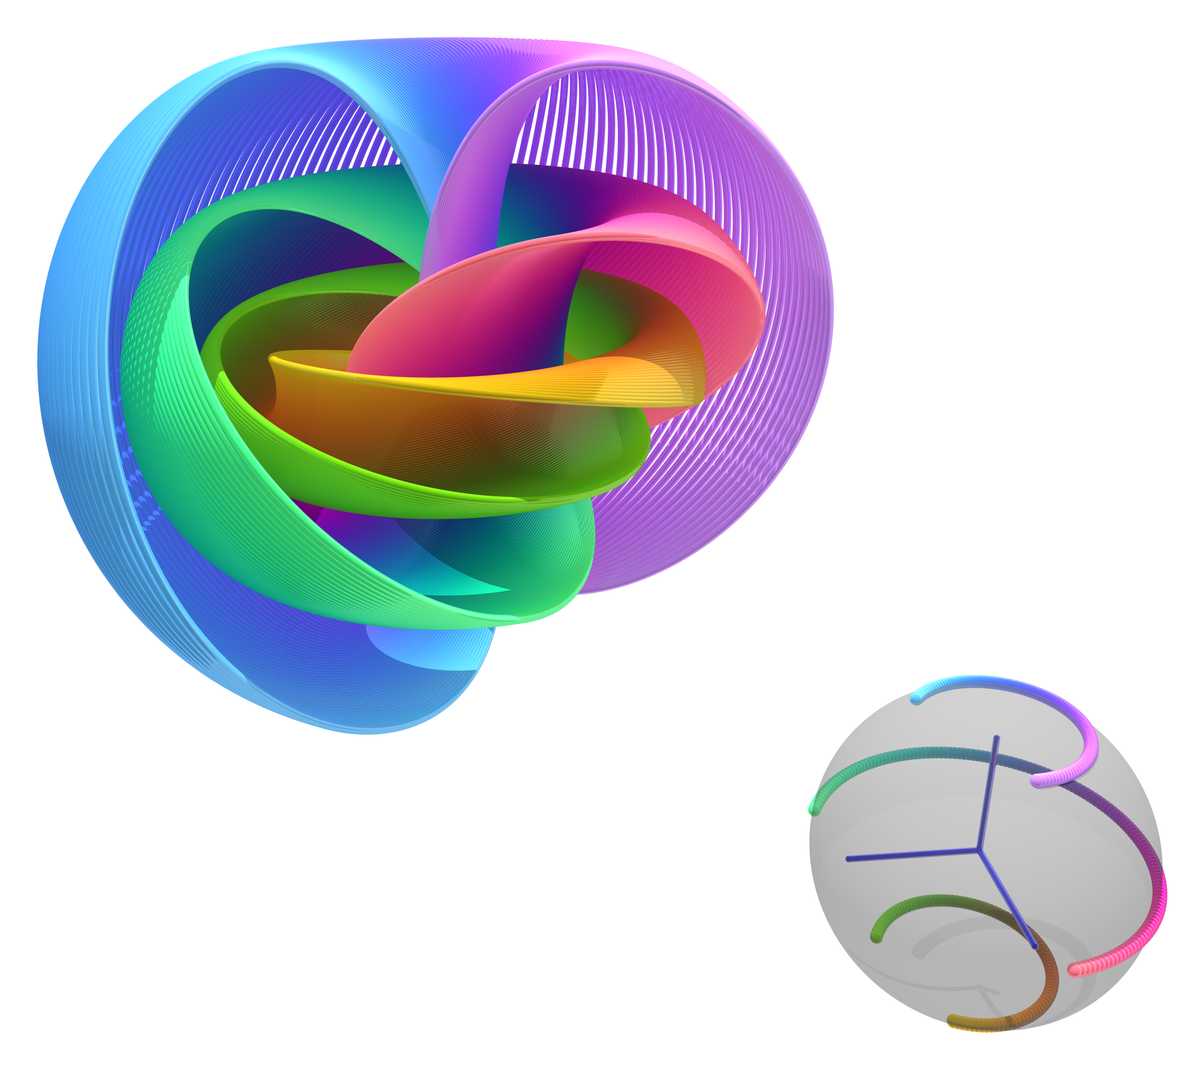
\includegraphics[width=9cm]{Hopf_Fibration.png}
        \caption{Fibres (or loops $\sim S^1$) of distinct points in the image are always linked, which happens to be a reason for Hopf maps to not be nullhomotopic, for unlinking them without making them intersect is impossible. Hence two points in the image of Hopf map can never be contracted to a common point continuously.}
        \end{figure}
    \item \textbf{M\"obius Band}, $$[0,1]^2/[(0,y)\sim(1,1-y)] \longrightarrow [0,1]$$
\begin{figure}[htp]
            \centering
            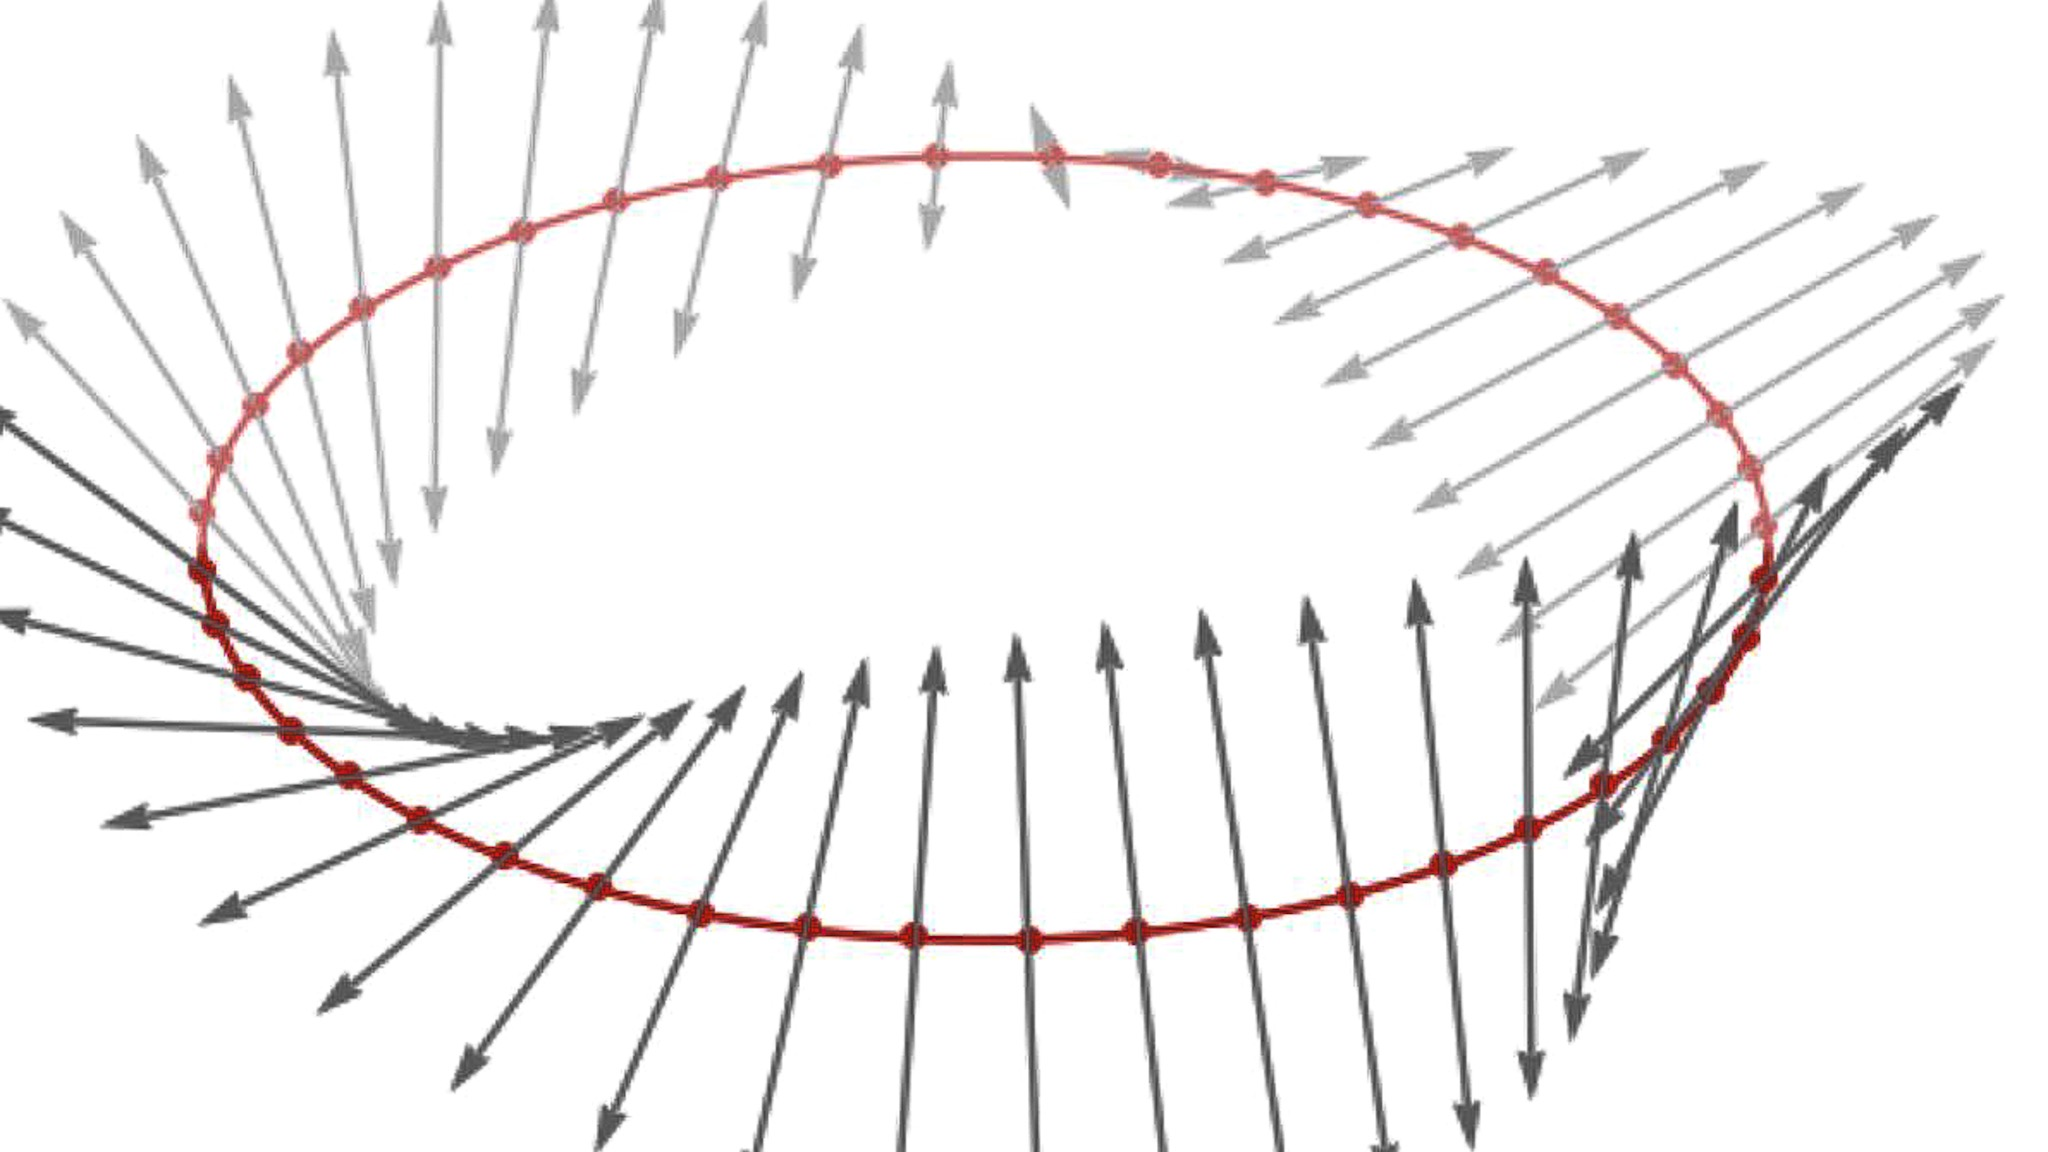
\includegraphics[width=9cm]{Universal_line_bundle.jpg}
            \caption{First example of a twisted or non-trivial bundle.}
        \end{figure}
        \item Let $\eta = (E, B, F, p)$ and $\eta' = (E', B', F', p')$, then $\eta\times\eta' := (E\times E', B\times B', F\times F', p\times p')$ is a fibre bundle, called the \textbf{product bundle}.
\end{enumerate}


\underline{\textbf{General Examples of Fibre Bundles:-}}

\underline{(I) \textbf{Principal $G$-Bundle}}:- A locally trivial bundle over $B$ with structure group and fibre equal to $G$, where the action of $G$ on $F$ is that of left translation, is called a \textbf{principal $G$-bundle over $B$}. 

In the sense that a left translation is the most rudimentary non-trivial action of $G$ among elements in $\text{Hom}_{\text{Grps}}\big(G, \text{Aut}(F)\big)$; principal $G$-bundles are the most primitive forms of fibre bundles in $H^1\big(B; \text{Aut}_{\text{Top}}(G)\big)$. It is perhaps owing to this nature that one finds twisted (or non-trivial) principal bundles iff the fibre sequence of pointed spaces:-

\begin{equation*}
    0\rightarrow G \hookrightarrow E \twoheadrightarrow B \rightarrow 0 \tag{† †}
\end{equation*}\\

splits towards the right as attested by the theorem below. Note that if the spaces involved had additional structure (say that of a $\mathbb{Z}$-module), then $(\dagger \dagger)$ would be split exact, (i.e.) $(E, B, G, p)$ would be trivial. But as pointed spaces are far from being algebraic objects, the phenomenon below is not expected at all.


\subsection*{Theorem 2.1} A principal $G$-bundle $(E, B, G, p)$ is trivial iff there exists a map $s: B \rightarrow E$ such that $p\circ s \equiv \text{id}_B$ (such maps are called \textbf{section maps}).

\textit{Proof.}
We shall prove this in three steps, each important on its own.\\


STEP 1:- (\underline{$E$ is a right $G$-space}). Define,
$$\psi: E\times G \rightarrow E$$
as follows,
$$\psi(z, g) = \psi(\varphi_{\alpha}(x,f), g):= \varphi_{\alpha}(x, f\cdot g)$$


Let's first establish that $\psi$ is well-defined. Say, $z = \varphi_{\alpha}(x, f) = \varphi_{\beta}(x, f')$. Then,\\
$$(x, f) = \varphi_{\alpha}^{-1}\circ\varphi_{\beta}(x, f') = \varphi_{\alpha\beta}(x, f') = \big(x, \widetilde{\varphi}_{\alpha\beta}(x)(f')\big)$$

$$(x, f\cdot g) = \big(x, [\widetilde{\varphi}_{\alpha\beta}(x)(f')]\cdot g\big)$$


Now as $\widetilde{\varphi}_{\alpha\beta}(x)$ is a left translation by some $g' \in G$, we have,
\begin{equation*}
\begin{split}
(x, f\cdot g) & = \big(x, (g'\cdot f')\cdot g\big) = \big(x, g'\cdot (f'\cdot g)\big) \\ 
 & = \big(x, \widetilde{\varphi}_{\alpha\beta}(x)(f'\cdot g)\big) 
\end{split}
\end{equation*}
Therefore,
$$\varphi_{\alpha}(x, f\cdot g) = \varphi_{\beta}(x, f\cdot g)$$


As the map, $\big((x, f), g\big) \in \big(U_{\alpha}\times G\big)\times G \longrightarrow (x, f\cdot g) \in U_{\alpha}\times G$ is continuous, $\psi\big|_{p^{-1}(U_{\alpha})}$ is continuous, and hence by gluing lemma $\psi$ is a continuous right action. In particular, $$\big(\varphi_{\alpha}(x, f)\big)\cdot g = \varphi_{\alpha}(x, f\cdot g)$$  \\
STEP 2:- (\underline{Equivariant Bundle Morphisms are Isomorphisms})\\


We shall now show that two principal $G$-bundles over $B$ are isomorphic iff they are isomorphic as right $G$-spaces. Let $E$, $E'$ be the total spaces of the isomorphic principal bundles. Passing onto the common refinement of locally trivializing cover, $E \cong E'$ $\implies$ $\exists$ $h_{\alpha}: U_{\alpha}\times F \rightarrow U_{\alpha}\times F$ homeomorphisms. Clearly by STEP 1,
$$h_{\alpha}\big((x, f)\cdot g\big) = h_{\alpha}(x, fg) = \big(x, \widetilde{h}_{\alpha}(x)(fg)\big) = \big(x, \widetilde{h}_{\alpha}(x)(f)\cdot g\big) = \big(x, \widetilde{h}_{\alpha}(x)(f)\big)\cdot g = \big(h_{\alpha}(x, f)\big)\cdot g$$

As $\varphi_{\alpha}$ is an isomorphism of right $G$-spaces $U_{\alpha}\times F$ and $p^{-1}(U_{\alpha})$, we have that,
$$\varphi_{\alpha}\circ h_{\alpha}\circ \varphi_{\alpha}^{-1}: p^{-1}(U_{\alpha}) \rightarrow (p')^{-1}(U_{\alpha})$$
is an isomorphism of right $G$-spaces. This implies, $\psi\big|_{p^{-1}(U_{\alpha})}$ is an isomorphism of right $G$-spaces. 


Now, $\psi$ being a homeomorphism and a morphism of right $G$-spaces locally, is a global isomorphism of right $G$-spaces $E$ and $E'$

Conversely, suppose $\psi$ is morphism of right $G$-spaces, (i.e.) a continuous map satisfying, $$\psi(z\cdot g) = \psi(z)\cdot g$$ Clearly, $\varphi_{\alpha}^{-1}\circ \psi\circ \varphi_{\alpha}$ is fibre preserving, so if,
$$\varphi_{\alpha}^{-1}\circ \psi\circ \varphi_{\alpha}(x, g) = \big(x, A_{\alpha}(x, g)\big)$$
then,
$$\varphi_{\alpha}^{-1}\circ \psi\circ \varphi_{\alpha}(x, e)\cdot g = \big(x, A_{\alpha}(x, e)\cdot g\big) = \varphi_{\alpha}^{-1}\circ \psi\circ \varphi_{\alpha}(x, g)$$
Set, 
$$\widetilde{h}_{\alpha}(x):= A_{\alpha}(x, e)$$
$$h_{\alpha}(x, g) := \big(x, \widetilde{h}_{\alpha}(x)g\big)$$
the required set of homeomorphisms.

STEP 3:- (\underline{Sections to Global Trivializations})

A principal $G$-bundle $(E, B, G, p)$ is trivial in $H^{1}\big(B; \text{Aut}(F)\big)$ iff $E\cong B\times F$. Given a section map $s: B \rightarrow E$, define,
$$\psi: B\times F \rightarrow E$$
$$\psi(b,g):= s(b)\cdot g$$
Note that,
$$p\big(s(b)\cdot g\big) = b$$
which implies $\psi$ is fibre preserving and a morphism of right $G$-spaces, hence an isomorphism by STEP 2.

\underline{(II) \textbf{Ehresmann's Theorem}}:- Let $F: X \rightarrow Y$ be a proper submersion of smooth manifolds and $y \in Y$, then $(X, Y, F^{-1}(y), F)$ is a fibre bundle.
\textit{Proof.}
Since the fibration is defined locally, one can assume WLOG that $Y= \mathbb{R}^n$. Let $F: X\rightarrow Y$ be a submersion, we have to show $F^{-1}(Y)\cong Y\times F^{-1}(0) = \mathbb{R}^n\times F^{-1}(0)$. On $Y$ we have the vector-fields $\frac{\partial}{\partial x_i}$ $(1\leq i\leq n)$. Let $\varphi_{X_i}^t$ denote the integral curves of the $X_i$, where $X_i$ are vector-fields $F$-related to $\frac{\partial}{\partial x_i}$. Since the integral curves $\varphi_{\frac{\partial}{\partial x_i}}^t$ are defined $\forall t\in (-\infty, \infty)$, so are the curves $\varphi_{X_i}^t$. Define, 
$$G: F^{-1}(\mathbb{R}^n)\rightarrow \mathbb{R}^n\times F^{-1}(0)$$
$$G(z):= \big(F(z), \varphi_{X_n}^{-t_n}\circ\cdots \circ \varphi_{X_1}^{-t_1}(z)\big)$$
Note that $G$ has a well-defined inverse,
$$G^{-1}(t_1, \ldots, t_n, x) = \varphi_{X_n}^{t_1}\circ\cdots \circ \varphi_{X_1}^{t_n}(x)$$
$G$ is smooth as $F$ and $\varphi_{X_i}^t$ are smooth $(1\leq i\leq n)$. So, $G$ is a diffeomorphism, (i.e.) the bundle is locally trivial.

\subsection*{Remark 2}
    Basically, the fibres on each $x\in \mathbb{R}^n$ are being moved to $F^{-1}(0)$ via integral curves that are $F$-related to $\frac{\partial}{\partial x_i}$. For more, see \cite{guillemin2010differential}


\underline{\textbf{Corollaries to Ehresmann's Theorem}}:-

\begin{enumerate}[(i)]
    \item $G$ a compact Lie group, $X$ a smooth manifold with free action of $G$, then $\big(X, X/G, G, X\rightarrow X/G\big)$ is a fibre bundle\footnote{Quotient Manifold Theorem will tell you that the setup satisfies the hypothesis necessary for applying Ehresmann's Theorem.}.
    \item $G$ a Lie group, $H$ a compact subgroup of $G$, then $\big(G, G/H, H, G\rightarrow G/H\big)$ is a fibre bundle.
\end{enumerate}

One can use (II) to construct bundles with classical spaces like $\mathbb{CP}^n$, $\mathbb{HP}^n$, $\mathbb{RP}^n$, $U(n)$, $SO(n)$, $SU(n)$, $S^n$, $G(n,k)$, $V(n,k)$ (\textbf{Stiefel manifold}), and more. We compile them here:-

\begin{itemize}
    \item $\big(O(n), S^{n-1}, O(n-1), O(n) \rightarrow O(n)/O(n-1)\big)$ 
    \item $\big(V(n, k), G(n,k), O(k), V(n,k) \rightarrow V(n,k)/O(k)\big)$
    \item $\big(O(n), G(n,k), O(k)\times O(n-k), O(n)\rightarrow O(n)/(O(k)\times O(n-k)\big)$
\end{itemize}


One can similarly write the complex and quaternionic analogues of the above. For $n=\infty$, the second bundle in the list is called the \textbf{universal bundle} corresponding to the group $GL_k(\mathbb{R})$.

Having introduced fibre bundles, it is time to see means to operate with these, (i.e.) construct new ones from old. There are two general ways of constructing new bundles:-
\begin{enumerate}[(i)]
    \item Continuous Maps 
    \item Group Homomorphisms
\end{enumerate}
\underline{\textbf{(I) Pullback Bundle}}

Let $(E, B, F, p)$ be a fibre bundle and $f: B'\rightarrow B$ be a continuous map, then the bundle $(E', B', F, p')$ is defined via the following pullback square:-

$$\begin{tikzcd}
    E' := E\cross_B B' \arrow[hookrightarrow]{r} \arrow[d, "p'"'] &E \arrow[d, "p"]\\ B' \arrow[r, "f"'] & B
\end{tikzcd}$$


$$E' := \{(e, b')\in E\times B' |  p(e) = f(b')\}$$
$$p'(e, b'):= b'$$

\underline{Local Trivialization for $E'$}

If $\{(U_{\alpha}, \varphi_{\alpha})\}_{\alpha}$ trivialize $E$, then set, 
$$\widehat{U}_{\alpha}:= f^{-1}(U_{\alpha})$$
$$\widehat{\varphi}_{\alpha}: \widehat{U}_{\alpha}\times F \rightarrow E'$$
$$\widehat{\varphi}_{\alpha}(b', v):= (\varphi_{\alpha}(f(b'), v), b')\in E'$$


Note that, $(\widehat{\varphi}_{\alpha})^{-1}(e, b') = (b', \pi_2(\varphi_{\alpha}^{-1}(e)))$ is an inverse of $\widehat{\varphi}_{\alpha}$. Hence, $\{(\widehat{U}_{\alpha}, \widehat{\varphi}_{\alpha})\}_{\alpha}$ trivialize $E'$. Another way to construct the total space $E'$ would be to modify the transition functions like so:-
$$\big\{\{\varphi_{\alpha\beta}\}_{\alpha, \beta}  |   \widetilde{\varphi}_{\alpha\beta}:U_{\alpha}\cap U_{\beta} \rightarrow G\big\} \rightarrow \big\{\{\widehat{\varphi}_{\alpha\beta}\}_{\alpha, \beta}  |   \widetilde{\widehat{\varphi}}_{\alpha\beta}:U_{\alpha}\cap U_{\beta} \rightarrow G\big\}$$
The new bundle $\eta' = (E', B', F, p')$ is denoted by $f^*\eta$ where $\eta = (E, B, F, p)$, and is called the \textbf{pullback of the bundle $\eta$}.

If $B'\xhookrightarrow{i} B$ is an inclusion, then $i^*\eta$ is called the \textbf{restriction bundle}.

\underline{\textbf{(II) Structure Group Alteration}}

Let $\rho: G\rightarrow G'$ be a continuous group homomorphism, and $(E, B, F, p)$ be a bundle with gauge group $G$. Then the following modification of the transition functions yields a new bundle:-
$$\{\widetilde{\varphi}_{\alpha\beta}\}_{\alpha, \beta} \rightarrow \{\rho\circ\widetilde{\varphi}_{\alpha\beta}\}_{\alpha, \beta}$$
The group action of $\text{Im}(\rho)$ on $F$ is clear. One has to check that $\{\rho\circ\widetilde{\varphi}_{\alpha\beta}\}_{\alpha, \beta}$ is a cocycle in $H^1(B; G')$, for this, we exploit here the fact that $\rho$ is a group homomorphism to get:-
$$\big(\rho\circ\widetilde{\varphi}_{\alpha\beta}\big)\circ \big(\rho\circ\widetilde{\varphi}_{\beta\gamma}\big) \circ \big(\rho\circ\widetilde{\varphi}_{\gamma\alpha}\big) = \rho\circ\big(\widetilde{\varphi}_{\alpha\beta}\circ \widetilde{\varphi}_{\beta\gamma}\circ \widetilde{\varphi}_{\gamma\alpha}\big) = \rho(e) = e'$$
$$\rho\circ\big(\widetilde{\varphi}_{\alpha\alpha}\big) = \rho(e) = e'$$
where $e$, $e'$ are identity elements in $G$, $G'$, respectively. 


Let $\eta = (E, B, F, p)$, then the new bundle induced by the gauge group homomorphism shall be denoted by $\rho(\eta)$.
% BLOG-CONTENT-END
\bibliographystyle{amsalpha}
\bibliography{tools/profiles/k-theory/references}
\end{document}
